\subsection{Extension to nervous-system networks: supported routes and dispersed arrival}\label{sec:nervous-network}
The same architecture can represent a local, calibrated approximation to signaling between sensory, spinal, brainstem, cortical, or motor populations. Its variables are population features or small perturbations about a fixed operating state, not individual action potentials. The map describes a functional input--output projection; anatomical axonal projection alone does not identify that map. A constant-gain window is sufficient for the following extension, so oscillatory phase gating is optional. Chemical synapses, electrical coupling, refractory effects, and neuromodulatory state can require distinct kernels or nonlinear state equations outside this approximation.

The biological motivation is concrete. Auditory-brainstem experiments show that nodal and internodal geometry changes conduction timing \citep{ford2015}. Human PFC--M1 recordings support selective population-subspace transfer \citep{binish2026}. These observations motivate separate timing and projection quantities; neither establishes their particular combination here. In a sensorimotor return, muscle mechanics and sensory transduction also intervene. Those stages require calibrated operators and causal kernels rather than an additional unexplained ``communication delay.''

\paragraph{One network operator.} Let $N$ be the number of populations and $x_i(t)\in\R^{n_i}$ the perturbation features at population $i$. On each directed edge $j\to i$, let $L_{ij}:\R^{n_j}\to\R^{n_i}$ include its fixed nonnegative gate gain and its possibly signed translation map. Let $\tau_{ij}\ge\tau_{\min}>0$ be conduction time, and let $h_{ij}$ be a causal probability measure for residual processing. Densities recover Eq.~\eqref{eq:transfer}; a unit point mass recovers the ideal discrete-delay loop. With zero prehistory, define
\begin{equation}
x_i(t)=b_i(t)+\sum_{j:j\to i}\int_{[0,\infty)}L_{ij}x_j(t-\tau_{ij}-s)\,dh_{ij}(s).
\label{eq:network-transfer}
\end{equation}
Here $b_i$ is externally supplied content, not an unobserved recurrence term. The positive lower bound on edge conduction excludes instantaneous algebraic cycles. A useful sufficient bounded-signal stability condition is
\[
\rho_*:=\max_i\sum_{j:j\to i}\|L_{ij}\|<1,
\]
using the maximum of the population Euclidean norms. It is sufficient, not necessary, and stronger than some two-population stability conditions above.

For a directed walk $w=(j=i_0,i_1,\ldots,i_m=i)$, possibly visiting a population repeatedly, define its ordered translation, conduction sum, and processing measure by
\[
 L_w=L_{i_m i_{m-1}}\cdots L_{i_1i_0},\qquad
 \tau_w=\sum_{a=1}^m\tau_{i_ai_{a-1}},\qquad
 h_w=h_{i_mi_{m-1}}*\cdots*h_{i_1i_0}.
\]
For a source step $b_j(t)=d\mathbf1_{t\ge0}$, with content contrast $d\in\R^{n_j}$ and all other external inputs zero, set
\[
 F_w(t)=h_w([0,t-\tau_w])
\]
when $t\ge\tau_w$, and $F_w(t)=0$ otherwise. This cumulative processing response lies in $[0,1]$. A target readout $v\in\R^{n_i}$ is fixed independently of the tested trials.

\begin{theorem}[Supported-route arrival and threshold certificates]\label{thm:network}
For $i\ne j$, Eq.~\eqref{eq:network-transfer} has the unique causal solution
\begin{equation}
x_i(t)=\sum_{w:j\rightsquigarrow i}L_wd\,F_w(t),\qquad
 y_v(t)=v^\top x_i(t)=\sum_{w:j\rightsquigarrow i}c_wF_w(t),\quad c_w=v^\top L_wd.
\label{eq:walk-response}
\end{equation}
Only walks of length at most $\lfloor t/\tau_{\min}\rfloor$ can contribute at a finite time. Let $s_w=\inf\operatorname{supp}h_w$, and let
\[
 D_* =\inf_{w:c_w\ne0}(\tau_w+s_w),
\]
with $D_*=\infty$ when every coefficient is zero. Then:
\begin{enumerate}[label=(\roman*),leftmargin=*]
\item No target readout occurs before $D_*$. In particular, a faster anatomical route with $c_w=0$ cannot determine this item's readout onset. If every $c_w=0$, timing changes alone cannot create readout support while the maps remain fixed.
\item For instantaneous processing, aggregate walks with the same arrival time $D$ into $C_D=\sum_{w:\tau_w=D}c_w$. The first nonzero readout jump occurs at the smallest $D$ with $C_D\ne0$, if such a $D$ exists. A nonzero individual route is therefore not sufficient for an observed onset at its arrival time.
\item Define $B_v(t)=\sum_w|c_w|F_w(t)$. For an absolute readout threshold $\vartheta>0$, $B_v(t)<\vartheta$ certifies no completion at time $t$. For any selected walk $w_0$,
\[
 |y_v(t)|\ge |c_{w_0}|F_{w_0}(t)-\sum_{w\ne w_0}|c_w|F_w(t).
\]
If this lower bound is at least $\vartheta$, completion has occurred by $t$. These certificates permit signed maps, unequal delays, dispersion, and cancellation.
\end{enumerate}
Under $\rho_*<1$, the walk sum is also absolutely convergent uniformly for bounded source steps, and the bounded causal solution is unique on the entire time axis.
\end{theorem}
\begin{proof}
Write $\mathcal K$ for the edge-integral operator in Eq.~\eqref{eq:network-transfer}. Substituting $x=b+\mathcal Kx$ repeatedly gives
\[
 x=\sum_{m=0}^{M}\mathcal K^m b+\mathcal K^{M+1}x.
\]
Every application of $\mathcal K$ retards an argument by at least $\tau_{\min}$. Consequently the remainder vanishes at a fixed time $t$ as soon as $(M+1)\tau_{\min}>t$, using zero prehistory. The $m$th term expands over all length-$m$ directed walks. Ordered matrix multiplication gives $L_w$; integration of the scalar causal measures composes by convolution. Applied to a source step it yields $L_wd\,h_w([0,t-\tau_w])$. This proves Eq.~\eqref{eq:walk-response} and finite-time finiteness. The same substitution for the difference of two causal solutions makes that difference zero at each finite time, establishing uniqueness without a stability assumption.

A measure assigns no mass strictly below the infimum of its support. Thus every term with $c_w\ne0$ is zero for $t<\tau_w+s_w$; terms with zero coefficient vanish at every time. This proves (i), including the empty-set case. With point-mass processing, $F_w(t)=\mathbf1_{t\ge\tau_w}$. At any fixed arrival time the jump is therefore the finite sum $C_D$. If all earlier groups vanish, the readout before that time is zero, and its value after the jump is $C_D$. This proves (ii). The discrete arrival set is locally finite because of the positive edge-delay lower bound; hence any nonempty set of nonzero groups has a smallest member.

For (iii), apply the triangle inequality to the finite sum in Eq.~\eqref{eq:walk-response}; since $F_w\ge0$, the upper bound is exactly $B_v(t)$. Separate one term and apply the reverse triangle inequality to obtain the displayed lower bound. Meeting that sufficient lower bound implies the absolute readout meets threshold at $t$, whereas the upper-bound test excludes it at that time. It does not exclude an earlier transient crossing unless the upper-bound test holds throughout the earlier interval.

Finally, normalized measures and the block maximum norm imply $\|\mathcal K\|\le\rho_*$. The geometric series in $\mathcal K$ converges in operator norm when $\rho_*<1$. Expanding the series of edge norm products gives the scalar majorant $\|d\|\sum_{m\ge0}\rho_*^m$, which is finite. It bounds the summed norms of all vector walk contributions. Banach's contraction argument then supplies existence and uniqueness of the bounded solution. Stability is not asserted for networks failing this sufficient condition.
\end{proof}

\begin{lemma}[A less conservative weighted stability certificate]\label{lem:weighted-network}
Set $B_{ij}=\|L_{ij}\|$ on an edge and zero otherwise. If the spectral radius $\rho(B)<1$, Theorem~\ref{thm:network}'s uniform absolute convergence conclusion holds even when $\rho_*\ge1$. Equivalently, there are positive weights $q_i$ and $c<1$ such that $Bq\le cq$.
\end{lemma}
\begin{proof}
When $\rho(B)<1$, the matrix Neumann series converges and $q=(I-B)^{-1}\mathbf1=\sum_{m\ge0}B^m\mathbf1$ has every coordinate at least one. Thus $Bq=q-\mathbf1$ and $c=\max_i(1-1/q_i)<1$. In the weighted signal norm $\|x\|_q=\sup_{t,i}\|x_i(t)\|/q_i$, normalized processing measures give
\[
\|\mathcal Kx\|_q\le\max_i\frac{\sum_j B_{ij}q_j}{q_i}\|x\|_q\le c\|x\|_q.
\]
The geometric-series proof of Theorem~\ref{thm:network} now applies in this norm, also to the sum of the norms of walk contributions. Conversely, if $Bq\le cq$, the matrix $\operatorname{diag}(q)^{-1}B\operatorname{diag}(q)$ has row sums at most $c$. Its spectral radius, which equals $\rho(B)$, is at most $c<1$. This proves the equivalence and the certificate.
\end{proof}
For two scalar edge norms 2 and 0.4, the unweighted row bound is 2, whereas $\rho(B)=\sqrt{0.8}<1$; weights $(\sqrt5,1)$ recover the loop-product condition. Acyclic graphs have nilpotent $B$ and satisfy the weighted certificate regardless of individual finite edge gains. The criterion is exact for uniform absolute walk summability in the nonnegative scalar comparison network under unrestricted positive step forcing: its walk majorant is the matrix series $\sum_m B^m$, convergent exactly when $\rho(B)<1$. Signed maps and cancellations can yield bounded responses beyond this comparison condition, so it remains sufficient rather than necessary for the original network. Neither condition is needed for the finite-time causal construction.

\paragraph{How this extends the projection theorem.} Theorem~\ref{thm:inter} is the one-edge content contrast; Theorem~\ref{thm:reciprocal} selects alternating walks in a two-population loop; Theorem~\ref{thm:network} permits multiple intervening populations and competing routes. A direct null projection can coexist with an effective detour because the detour has a different map product. Conversely, a nonzero projection can remain below threshold or be canceled. The added latency is consequently item- and readout-specific. It is constrained by supported routes and their measured kernels, rather than a universal extra duration of unreported processing. With continuous processing densities, $D_*$ is a lower bound on arrival and need not be an attained nonzero event.

\paragraph{A test separating missing support from slow signaling.} Present two independently decoded source contrasts $d_1,d_2$ on the same anatomical route, freeze its maps, and estimate their arrival responses on held-out trials. The model permits $v^\top L_wd_1=0$ and $v^\top L_wd_2\ne0$ at the same conduction time. An additional supported detour can delay only the first contrast. Removing that detour should selectively remove its later response while preserving the second contrast's direct response. This requires an isolated intervention and a calibrated source contrast; ordinary cross-correlation cannot establish the route products.

\begin{proposition}[Dispersion and the conduction--processing ambiguity]\label{prop:dispersion}
Let an edge's residual causal processing time $S$ have finite mean $\mu$ and variance $\sigma_h^2$, and define $H(\Omega)=\mathbb E e^{-i\Omega S}$. At constant gain its temporal carrier factor is $e^{-i\Omega\tau}H(\Omega)$. Then
\begin{equation}
 |H(\Omega)-e^{-i\Omega\mu}|\le\tfrac12\Omega^2\sigma_h^2,
 \qquad |H(\Omega)|\ge\max\{0,1-\tfrac12\Omega^2\sigma_h^2\}.
\label{eq:dispersion-bound}
\end{equation}
Along a walk, convolution adds processing means and variances. Knowledge of the complete temporal response still does not generally separate conduction from an unconstrained processing kernel: if $S\ge u\ge0$ almost surely, replacing $(\tau,S)$ by $(\tau+u,S-u)$ leaves every temporal response unchanged.
\end{proposition}
\begin{proof}
Set $Z=S-\mu$, so $\mathbb EZ=0$ and $\mathbb EZ^2=\sigma_h^2$. For real $a$, the integral Taylor remainder of $e^{-ia}$ implies $|e^{-ia}-1+ia|\le a^2/2$. Therefore
\[
 |\mathbb E e^{-i\Omega Z}-1|
 =|\mathbb E(e^{-i\Omega Z}-1+i\Omega Z)|
 \le\tfrac12\Omega^2\mathbb EZ^2.
\]
Multiplication by $e^{-i\Omega\mu}$ proves the first bound. The reverse triangle inequality proves the second, with zero included because magnitude is nonnegative. A convolution of probability measures is the law of a sum of independent variables with those measures. Its mean is the sum of the means and its variance is the sum of the variances, proving the walk statement; dependence would require a different joint delay model. Finally, $\tau+u+(S-u)=\tau+S$ pointwise. The shifted variable remains causal by the assumed support gap. Thus its total impulse measure, Fourier transform, and responses to arbitrary inputs are identical. This last equivalence concerns constant-gain temporal operators; changing a time-varying gate requires a separate invariance argument.
\end{proof}

Dispersion can reduce carrier magnitude without removing structural support. For a causal uniform residual delay on $[\mu-a,\mu+a]$, $0<a\le\mu$, the exact magnitude is $|\sin(\Omega a)/(\Omega a)|$. Width is therefore an additional measurable quantity, not interchangeable with the mean delay or a null projection. Separating physiological travel time from synaptic integration needs a kernel constraint, two-site timing measurement, or another independent calibration even with broadband recordings.

\paragraph{Sharpness, other kernels, and independent timing.} The coefficient $1/2$ in Eq.~\eqref{eq:dispersion-bound} is asymptotically sharp. With $Z=S-\mu$ and finite second moment, dominated convergence applied to the second-order remainder gives $\mathbb E e^{-i\Omega Z}=1-\Omega^2\sigma_h^2/2+o(\Omega^2)$. For $\sigma_h^2>0$, the ratio of the first bound's two sides tends to one as $\Omega\to0$; a smaller universal coefficient is impossible. This does not assert equality at a nonzero frequency, and the lower magnitude bound becomes uninformative at sufficiently high frequency. For an exponential causal kernel of mean $\mu$, $H(\Omega)=(1+i\Omega\mu)^{-1}$ and $|H|=(1+\Omega^2\mu^2)^{-1/2}$; the same bound applies although this kernel is not uniform.

The ambiguity is broken by an independently known processing kernel, or by an imposed zero lower endpoint of its support together with resolved onset on an isolated, nonzero pathway: the lower endpoint of the total impulse measure is then $\tau$. An operational threshold crossing need not equal that endpoint. Two-site timing cancels downstream processing only when the two measurements share the same downstream stages and the measured interval isolates travel between the sites. Additional unknown stages restore ambiguity. Broadband measurements alone identify the total temporal operator, not its unconstrained decomposition. Supplement S20 gives non-uniform-kernel checks and numerical power calculations.

\paragraph{Faster travel need not mean earlier completion.} In an isolated scalar channel with unit source contrast, translation magnitude 0.5, $\psi=0$, $\kappa=2$, and a 40 Hz carrier, choose $\alpha=-\Omega(0.018)$ so that 18 ms conduction is aligned. Threshold 0.4 is met at the initial arrival in the instantaneous-processing step model. Shortening conduction to 13 ms with preference fixed produces $|\Delta|=0.4\pi$ and amplitude $0.5\exp[2(\cos(0.4\pi)-1)]\approx0.126$, which never reaches that threshold without another input or alignment change. Compensating preference by the opposite phase shift restores amplitude 0.5 and completion at 13 ms. This is a conditional content-by-timing prediction, not a claim that changing myelin affects only conduction. It links the identifiability calibration directly to the network's completion test: measured timing and calibrated gain must jointly predict the response.

\begin{figure}[htbp]\centering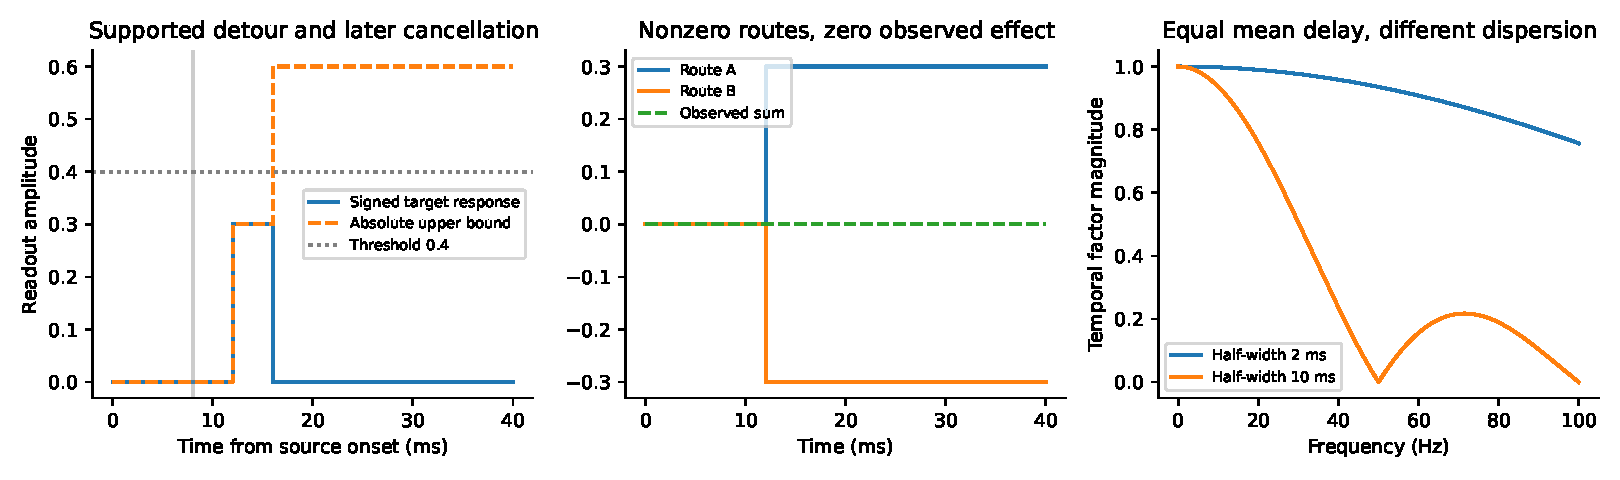
\includegraphics[width=.98\linewidth]{figure_nervous_network.pdf}\caption{Synthetic nervous-network illustrations; the separate randomized verification uses 100 networks with four populations and two features per population. Left: a fast 8 ms route has zero item projection, while a supported detour arrives at 12 ms. An opposing 16 ms route cancels the sustained readout. Middle: equal and opposite simultaneous route contributions cancel completely. Right: normalized causal uniform processing kernels with the same 15 ms mean and half-widths 2 and 10 ms retain different carrier magnitudes. These are model consequences, not measured physiological delays.}\label{fig:nervous-network}\end{figure}
